\documentclass[runningheads]{llncs}

\usepackage{fontspec}
\setmainfont{Times New Roman}
\usepackage{amsmath,amssymb}
\usepackage{graphicx}
\usepackage{booktabs}
\usepackage{xcolor}
\usepackage{listings}
\usepackage[hidelinks]{hyperref}

\renewcommand{\contentsname}{Mục lục}
\setcounter{tocdepth}{2}

\lstset{
  language=Python,
  basicstyle=\ttfamily\scriptsize,
  keywordstyle=\color{blue!70!black},
  commentstyle=\color{green!40!black},
  stringstyle=\color{red!60!black},
  numbers=none,
  frame=single,
  rulecolor=\color{black!25},
  backgroundcolor=\color{gray!5},
  breaklines=true,
  breakatwhitespace=false,
  columns=fullflexible,
  keepspaces=true,
  showstringspaces=false,
  xleftmargin=4pt,
  xrightmargin=4pt,
  aboveskip=6pt,
  belowskip=6pt
}

\begin{document}

\title{Bài 3: Linear Regression}
\author{Vũ Hữu Tiệp\thanks{Bài làm sao chép theo bài viết trên trang
\url{https://machinelearningcoban.com/2016/12/28/linearregression/}
của tác giả Vũ Hữu Tiệp. Đây là bài tập thực hành latex của SV
Vũ Quí Đức 26120072 CNTN26, Khoa CNTT, Trường ĐH KHTN TPHCM.}}
\institute{Machine Learning cơ bản}

\makeatletter
\let\originaladdcontentsline\addcontentsline
\renewcommand{\addcontentsline}[3]{%
  \def\@tempa{#2}%
  \def\@tempb{title}%
  \ifx\@tempa\@tempb
  \else
    \def\@tempb{author}%
    \ifx\@tempa\@tempb
    \else
      \originaladdcontentsline{#1}{#2}{#3}%
    \fi
  \fi
}
\maketitle
\let\addcontentsline\originaladdcontentsline
\makeatother

\begin{abstract}
Bài viết giới thiệu Linear Regression (hồi quy tuyến tính), một thuật toán
Supervised Learning cơ bản. Nội dung trình bày cách xây dựng mô hình, sai số
dự đoán, hàm mất mát, nghiệm theo phương trình chuẩn và giả nghịch đảo, cùng
ví dụ minh họa bằng Python và scikit-learn.
\keywords{Linear Regression \and hồi quy tuyến tính \and hàm mất mát \and
giả nghịch đảo \and Machine Learning.}
\end{abstract}

\clearpage
\tableofcontents
\clearpage

\section{Giới thiệu}

Quay lại ví dụ đơn giản được nêu trong bài trước: một căn nhà rộng
$x_1~\text{m}^2$, có $x_2$ phòng ngủ và cách trung tâm thành phố
$x_3~\text{km}$ có giá là bao nhiêu. Giả sử chúng ta đã có số liệu thống kê
từ 1000 căn nhà trong thành phố đó, liệu rằng khi có một căn nhà mới với các
thông số về diện tích, số phòng ngủ và khoảng cách tới trung tâm, chúng ta có
thể dự đoán được giá của căn nhà đó không? Nếu có thì hàm dự đoán
$y = f(\mathbf{x})$ sẽ có dạng như thế nào. Ở đây
$\mathbf{x} = [x_1, x_2, x_3]$ là một vector hàng chứa thông tin \emph{input},
$y$ là một số vô hướng (scalar) biểu diễn \emph{output} (tức giá của căn nhà
trong ví dụ này).

\textbf{Lưu ý về ký hiệu toán học:} trong các bài viết của tác giả, các số vô
hướng được biểu diễn bởi các chữ cái viết ở dạng không in đậm, có thể viết
hoa, ví dụ $x_1, N, y, k$. Các vector được biểu diễn bằng các chữ cái thường
in đậm, ví dụ $\mathbf{y}, \mathbf{x}_1$. Các ma trận được biểu diễn bởi các
chữ viết hoa in đậm, ví dụ $\mathbf{X}, \mathbf{Y}, \mathbf{W}$.

Một cách đơn giản nhất, chúng ta có thể thấy rằng: i) diện tích nhà càng lớn
thì giá nhà càng cao; ii) số lượng phòng ngủ càng lớn thì giá nhà càng cao;
iii) càng xa trung tâm thì giá nhà càng giảm. Một hàm số đơn giản nhất có thể
mô tả mối quan hệ giữa giá nhà và 3 đại lượng đầu vào là:
\begin{equation}
\label{eq:model}
y \approx f(\mathbf{x}) = \hat{y}, \qquad
f(\mathbf{x}) = w_1 x_1 + w_2 x_2 + w_3 x_3 + w_0,
\end{equation}
trong đó $w_1, w_2, w_3, w_0$ là các hằng số, $w_0$ còn được gọi là bias.
Mối quan hệ $y \approx f(\mathbf{x})$ bên trên là một mối quan hệ tuyến tính
(linear). Bài toán chúng ta đang làm là một bài toán thuộc loại regression.
Bài toán đi tìm các hệ số tối ưu $\{w_1, w_2, w_3, w_0\}$ chính vì vậy được
gọi là bài toán Linear Regression.

\textbf{Chú ý 1:} $y$ là giá trị thực của \emph{outcome} (dựa trên số liệu
thống kê chúng ta có trong tập \emph{training data}), trong khi $\hat{y}$ là
giá trị mà mô hình Linear Regression dự đoán được. Nhìn chung, $y$ và
$\hat{y}$ là hai giá trị khác nhau do có sai số mô hình, tuy nhiên, chúng ta
mong muốn rằng sự khác nhau này rất nhỏ.

\textbf{Chú ý 2:} \emph{Linear} hay \emph{tuyến tính} hiểu một cách đơn giản
là \emph{thẳng, phẳng}. Trong không gian hai chiều, một hàm số được gọi là
\emph{tuyến tính} nếu đồ thị của nó có dạng một \emph{đường thẳng}. Trong
không gian ba chiều, một hàm số được gọi là \emph{tuyến tính} nếu đồ thị của
nó có dạng một \emph{mặt phẳng}. Trong không gian nhiều hơn 3 chiều, khái
niệm \emph{mặt phẳng} không còn phù hợp nữa, thay vào đó, một khái niệm khác
ra đời được gọi là \emph{siêu mặt phẳng} (\emph{hyperplane}). Các hàm số
tuyến tính là các hàm đơn giản nhất, vì chúng thuận tiện trong việc hình dung
và tính toán. Chúng ta sẽ được thấy trong các bài viết sau, \emph{tuyến tính}
rất quan trọng và hữu ích trong các bài toán Machine Learning. Kinh nghiệm cá
nhân của tác giả cho thấy, trước khi hiểu được các thuật toán \emph{phi tuyến}
(non-linear, không phẳng), chúng ta cần nắm vững các kỹ thuật cho các mô hình
\emph{tuyến tính}.

\section{Phân tích toán học}

\subsection{Dạng của Linear Regression}

Trong phương trình \eqref{eq:model} phía trên, nếu chúng ta đặt
$\mathbf{w} = [w_0, w_1, w_2, w_3]^T$ là vector (cột) hệ số cần phải tối ưu
và $\bar{\mathbf{x}} = [1, x_1, x_2, x_3]$ (đọc là \emph{x bar} trong tiếng
Anh) là vector (hàng) dữ liệu đầu vào \emph{mở rộng}. Số $1$ ở đầu được thêm
vào để phép tính đơn giản hơn và thuận tiện cho việc tính toán. Khi đó,
phương trình \eqref{eq:model} có thể được viết lại dưới dạng:
\[
y \approx \bar{\mathbf{x}}\mathbf{w} = \hat{y}.
\]
Chú ý rằng $\bar{\mathbf{x}}$ là một vector hàng.

\subsection{Sai số dự đoán}

Chúng ta mong muốn rằng sự sai khác $e$ giữa giá trị thực $y$ và giá trị dự
đoán $\hat{y}$ (đọc là \emph{y hat} trong tiếng Anh) là nhỏ nhất. Nói cách
khác, chúng ta muốn giá trị sau đây càng nhỏ càng tốt:
\[
\frac{1}{2}e^2
= \frac{1}{2}(y - \hat{y})^2
= \frac{1}{2}(y - \bar{\mathbf{x}}\mathbf{w})^2,
\]
trong đó hệ số $\frac{1}{2}$ (\emph{lại}) là để thuận tiện cho việc tính toán
(khi tính đạo hàm thì số $\frac{1}{2}$ sẽ bị triệt tiêu). Chúng ta cần $e^2$
vì $e = y - \hat{y}$ có thể là một số âm, việc nói $e$ nhỏ nhất sẽ không đúng
vì khi $e = -\infty$ là rất nhỏ nhưng sự sai lệch là rất lớn. Bạn đọc có thể
tự đặt câu hỏi: \textbf{tại sao không dùng trị tuyệt đối $|e|$ mà lại dùng
bình phương $e^2$ ở đây?} Câu trả lời sẽ có ở phần sau.

\subsection{Hàm mất mát}

Điều tương tự xảy ra với tất cả các cặp \emph{(input, outcome)}
$(\mathbf{x}_i, y_i), i = 1, 2, \dots, N$, với $N$ là số lượng dữ liệu quan
sát được. Điều chúng ta muốn, tổng sai số là nhỏ nhất, tương đương với việc
tìm $\mathbf{w}$ để hàm số sau đạt giá trị nhỏ nhất:
\begin{equation}
\label{eq:loss}
\mathcal{L}(\mathbf{w})
= \frac{1}{2}\sum_{i=1}^N \left(y_i - \bar{\mathbf{x}}_i\mathbf{w}\right)^2.
\end{equation}
Hàm số $\mathcal{L}(\mathbf{w})$ được gọi là \textbf{hàm mất mát} (loss
function) của bài toán Linear Regression. Chúng ta luôn mong muốn rằng sự mất
mát (sai số) là nhỏ nhất, điều đó đồng nghĩa với việc tìm vector hệ số
$\mathbf{w}$ sao cho giá trị của hàm mất mát này càng nhỏ càng tốt. Giá trị
của $\mathbf{w}$ làm cho hàm mất mát đạt giá trị nhỏ nhất được gọi là
\emph{điểm tối ưu} (optimal point), ký hiệu:
\[
\mathbf{w}^\ast = \arg\min_{\mathbf{w}} \mathcal{L}(\mathbf{w}).
\]

Trước khi đi tìm lời giải, chúng ta đơn giản hóa phép toán trong phương trình
hàm mất mát \eqref{eq:loss}. Đặt
$\mathbf{y} = [y_1; y_2; \dots; y_N]$ là một vector cột chứa tất cả các
\emph{output} của \emph{training data};
$\bar{\mathbf{X}} = [\bar{\mathbf{x}}_1; \bar{\mathbf{x}}_2; \dots;
\bar{\mathbf{x}}_N]$ là ma trận dữ liệu đầu vào (mở rộng) mà mỗi hàng của nó
là một điểm dữ liệu. Khi đó hàm số mất mát $\mathcal{L}(\mathbf{w})$ được
viết dưới dạng ma trận đơn giản hơn:
\begin{equation}
\label{eq:loss-matrix}
\mathcal{L}(\mathbf{w})
= \frac{1}{2}\left\|\mathbf{y} - \bar{\mathbf{X}}\mathbf{w}\right\|_2^2,
\end{equation}
với $\|\mathbf{z}\|_2$ là Euclidean norm (chuẩn Euclid, hay khoảng cách
Euclid), nói cách khác $\|\mathbf{z}\|_2^2$ là tổng của bình phương mỗi phần
tử của vector $\mathbf{z}$. Tới đây, ta đã có một dạng đơn giản của hàm mất
mát được viết như phương trình \eqref{eq:loss-matrix}.

\subsection{Nghiệm cho bài toán Linear Regression}

\textbf{Cách phổ biến nhất để tìm nghiệm cho một bài toán tối ưu (chúng ta đã
biết từ khi học cấp 3) là giải phương trình đạo hàm (gradient) bằng 0!} Tất
nhiên đó là khi việc tính đạo hàm và việc giải phương trình đạo hàm bằng 0
không quá phức tạp. Thật may mắn, với các mô hình tuyến tính, hai việc này là
khả thi.

Đạo hàm theo $\mathbf{w}$ của hàm mất mát là:
\[
\frac{\partial \mathcal{L}(\mathbf{w})}{\partial \mathbf{w}}
= \bar{\mathbf{X}}^T\left(\bar{\mathbf{X}}\mathbf{w} - \mathbf{y}\right).
\]
Các bạn có thể tham khảo bảng đạo hàm theo vector hoặc ma trận của một hàm số
trong mục D.2 của tài liệu Matrix calculus. Đến đây tác giả xin quay lại câu
hỏi ở phần Sai số dự đoán phía trên về việc tại sao không dùng trị tuyệt đối
mà lại dùng bình phương. Câu trả lời là hàm bình phương có đạo hàm tại mọi
nơi, trong khi hàm trị tuyệt đối thì không (đạo hàm không xác định tại 0).

Phương trình đạo hàm bằng 0 tương đương với:
\begin{equation}
\label{eq:normal}
\bar{\mathbf{X}}^T\bar{\mathbf{X}}\mathbf{w}
= \bar{\mathbf{X}}^T\mathbf{y} \triangleq \mathbf{b}.
\end{equation}
Ký hiệu $\bar{\mathbf{X}}^T\mathbf{y} \triangleq \mathbf{b}$ nghĩa là
\emph{đặt} $\bar{\mathbf{X}}^T\mathbf{y}$ \emph{bằng} $\mathbf{b}$.

Nếu ma trận vuông $\mathbf{A} \triangleq \bar{\mathbf{X}}^T\bar{\mathbf{X}}$
khả nghịch (non-singular hay invertible) thì phương trình \eqref{eq:normal}
có nghiệm duy nhất: $\mathbf{w} = \mathbf{A}^{-1}\mathbf{b}$.

Vậy nếu ma trận $\mathbf{A}$ không khả nghịch (có định thức bằng 0) thì sao?
Nếu các bạn vẫn nhớ các kiến thức về hệ phương trình tuyến tính, trong trường
hợp này thì hoặc phương trình \eqref{eq:normal} vô nghiệm, hoặc là nó có vô
số nghiệm. Khi đó, chúng ta sử dụng khái niệm \emph{giả nghịch đảo}
(pseudo-inverse) $\mathbf{A}^{\dagger}$ (đọc là \emph{A dagger} trong tiếng
Anh). Giả nghịch đảo là trường hợp tổng quát của nghịch đảo khi ma trận không
khả nghịch hoặc thậm chí không vuông. Trong khuôn khổ bài viết này, tác giả
xin phép được lược bỏ phần này; bạn đọc quan tâm có thể xem thêm tài liệu về
Least Squares, Pseudo-Inverses, PCA \& SVD.

Với khái niệm giả nghịch đảo, điểm tối ưu của bài toán Linear Regression có
dạng:
\begin{equation}
\label{eq:solution}
\mathbf{w}
= \mathbf{A}^{\dagger}\mathbf{b}
= \left(\bar{\mathbf{X}}^T\bar{\mathbf{X}}\right)^{\dagger}
  \bar{\mathbf{X}}^T\mathbf{y}.
\end{equation}

\section{Ví dụ trên Python}

\subsection{Bài toán}

Trong phần này, tác giả chọn một ví dụ đơn giản về việc giải bài toán Linear
Regression trong Python, đồng thời so sánh nghiệm của bài toán khi giải theo
phương trình \eqref{eq:solution} và nghiệm tìm được khi dùng thư viện
scikit-learn của Python. Đây là thư viện Machine Learning được sử dụng rộng
rãi trong Python. Trong ví dụ này, dữ liệu đầu vào chỉ có 1 giá trị (1 chiều)
để thuận tiện cho việc minh họa trong mặt phẳng.

Chúng ta có một bảng dữ liệu về chiều cao và cân nặng của 15 người như dưới
đây:

\begin{table}[htbp]
\centering
\small
\caption{Dữ liệu chiều cao và cân nặng của 15 người.}
\label{tab:height-weight}
\begin{tabular}{cccc}
\toprule
Chiều cao (cm) & Cân nặng (kg) & Chiều cao (cm) & Cân nặng (kg) \\
\midrule
147 & 49 & 168 & 60 \\
150 & 50 & 170 & 72 \\
153 & 51 & 173 & 63 \\
155 & 52 & 175 & 64 \\
158 & 54 & 178 & 66 \\
160 & 56 & 180 & 67 \\
163 & 58 & 183 & 68 \\
165 & 59 &     &    \\
\bottomrule
\end{tabular}
\end{table}

Bài toán đặt ra là: liệu có thể dự đoán cân nặng của một người dựa vào chiều
cao của họ không? Trên thực tế, tất nhiên là không, vì cân nặng còn phụ thuộc
vào nhiều yếu tố khác nữa, thể tích chẳng hạn. Vì bài viết nói về các thuật
toán Machine Learning đơn giản nên tác giả giả sử rằng chúng ta có thể dự đoán
được.

Chúng ta có thể thấy là cân nặng sẽ tỉ lệ thuận với chiều cao (càng cao càng
nặng), nên có thể sử dụng Linear Regression model cho việc dự đoán này. Để
kiểm tra độ chính xác của model tìm được, chúng ta sẽ giữ lại cột 155 và 160
cm để kiểm thử, các cột còn lại được sử dụng để huấn luyện (train) model.

\subsection{Hiển thị dữ liệu trên đồ thị}

Trước tiên, chúng ta cần có hai thư viện numpy cho đại số tuyến tính và
matplotlib cho việc vẽ hình.

\noindent\begin{minipage}{\linewidth}\begin{lstlisting}
# To support both python 2 and python 3
from __future__ import division, print_function, unicode_literals
import numpy as np
import matplotlib.pyplot as plt
\end{lstlisting}\end{minipage}

Tiếp theo, chúng ta khai báo và biểu diễn dữ liệu trên một đồ thị.

\noindent\begin{minipage}{\linewidth}\begin{lstlisting}
# height (cm)
X = np.array([[147, 150, 153, 158, 163, 165, 168, 170, 173, 175, 178, 180, 183]]).T
# weight (kg)
y = np.array([[49, 50, 51, 54, 58, 59, 60, 62, 63, 64, 66, 67, 68]]).T
# Visualize data
plt.plot(X, y, 'ro')
plt.axis([140, 190, 45, 75])
plt.xlabel('Height (cm)')
plt.ylabel('Weight (kg)')
plt.show()
\end{lstlisting}\end{minipage}

\begin{figure}[htbp]
\centering
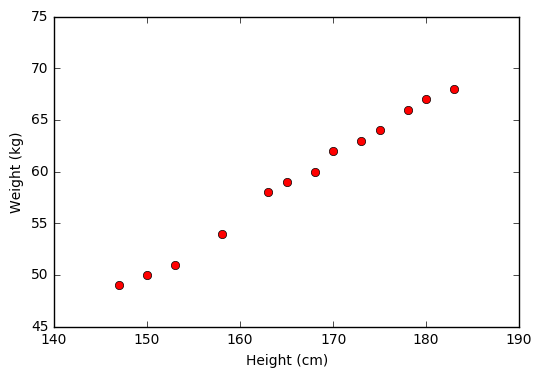
\includegraphics[width=0.72\textwidth]{images/output_3_0.png}
\caption{Biểu diễn dữ liệu chiều cao và cân nặng trên đồ thị.}
\label{fig:data}
\end{figure}

Từ đồ thị này ta thấy rằng dữ liệu được sắp xếp gần như theo một đường thẳng,
vậy mô hình Linear Regression nhiều khả năng sẽ cho kết quả tốt:
\[
\text{(cân nặng)} = w_1 \times \text{(chiều cao)} + w_0.
\]

\subsection{Nghiệm theo công thức}

Tiếp theo, chúng ta sẽ tính toán các hệ số $w_1$ và $w_0$ dựa vào công thức
\eqref{eq:solution}. Chú ý: giả nghịch đảo của một ma trận \texttt{A} trong
Python sẽ được tính bằng \texttt{numpy.linalg.pinv(A)}; \texttt{pinv} là từ
viết tắt của \emph{pseudo inverse}.

\noindent\begin{minipage}{\linewidth}\begin{lstlisting}
# Building Xbar
one = np.ones((X.shape[0], 1))
Xbar = np.concatenate((one, X), axis=1)

# Calculating weights of the fitting line
A = np.dot(Xbar.T, Xbar)
b = np.dot(Xbar.T, y)
w = np.dot(np.linalg.pinv(A), b)
print('w = ', w)

# Preparing the fitting line
w_0 = w[0][0]
w_1 = w[1][0]
x0 = np.linspace(145, 185, 2)
y0 = w_0 + w_1*x0

# Drawing the fitting line
plt.plot(X.T, y.T, 'ro')       # data
plt.plot(x0, y0)                # the fitting line
plt.axis([140, 190, 45, 75])
plt.xlabel('Height (cm)')
plt.ylabel('Weight (kg)')
plt.show()
\end{lstlisting}\end{minipage}

\noindent\begin{minipage}{\linewidth}\begin{lstlisting}
w =  [[-33.73541021]
 [  0.55920496]]
\end{lstlisting}\end{minipage}

\begin{figure}[htbp]
\centering
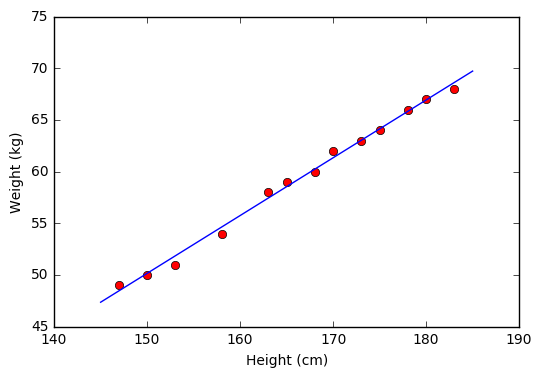
\includegraphics[width=0.72\textwidth]{images/output_5_1.png}
\caption{Đường thẳng hồi quy tuyến tính tìm được từ dữ liệu.}
\label{fig:fit}
\end{figure}

Từ đồ thị bên trên ta thấy rằng các điểm dữ liệu màu đỏ nằm khá gần đường
thẳng dự đoán màu xanh. Vậy mô hình Linear Regression hoạt động tốt với tập
dữ liệu \emph{training}. Bây giờ, chúng ta sử dụng mô hình này để dự đoán cân
nặng của hai người có chiều cao 155 và 160 cm mà chúng ta đã không dùng khi
tính toán nghiệm.

\noindent\begin{minipage}{\linewidth}\begin{lstlisting}
y1 = w_1*155 + w_0
y2 = w_1*160 + w_0

print(u'Predict weight of person with height 155 cm: %.2f (kg), real number: 52 (kg)' % (y1))
print(u'Predict weight of person with height 160 cm: %.2f (kg), real number: 56 (kg)' % (y2))
\end{lstlisting}\end{minipage}

\noindent\begin{minipage}{\linewidth}\begin{lstlisting}
Predict weight of person with height 155 cm: 52.94 (kg), real number: 52 (kg)
Predict weight of person with height 160 cm: 55.74 (kg), real number: 56 (kg)
\end{lstlisting}\end{minipage}

Chúng ta thấy rằng kết quả dự đoán khá gần với số liệu thực tế.

\subsection{Nghiệm theo thư viện scikit-learn}

Tiếp theo, chúng ta sẽ sử dụng thư viện scikit-learn của Python để tìm nghiệm.

\noindent\begin{minipage}{\linewidth}\begin{lstlisting}
from sklearn import datasets, linear_model

# fit the model by Linear Regression
regr = linear_model.LinearRegression(fit_intercept=False)  # fit_intercept = False for calculating the bias
regr.fit(Xbar, y)

# Compare two results
print('Solution found by scikit-learn  : ', regr.coef_)
print('Solution found by (5): ', w.T)
\end{lstlisting}\end{minipage}

\noindent\begin{minipage}{\linewidth}\begin{lstlisting}
    Solution found by scikit-learn  :  [[-33.73541021   0.55920496]]
    Solution found by (5):  [[-33.73541021   0.55920496]]
\end{lstlisting}\end{minipage}

Chúng ta thấy rằng hai kết quả thu được như nhau! Nghĩa là tác giả đã không
mắc lỗi nào trong cách tìm nghiệm ở phần trên. Source code Jupyter Notebook
cho bài này có tại
\url{https://github.com/tiepvupsu/tiepvupsu.github.io/blob/master/assets/LR/LR.ipynb}.

\section{Thảo luận}

\subsection{Các bài toán có thể giải bằng Linear Regression}

Hàm số $y \approx f(\mathbf{x}) = \mathbf{w}^T\mathbf{x}$ là một hàm tuyến
tính theo cả $\mathbf{w}$ và $\mathbf{x}$. Trên thực tế, Linear Regression có
thể áp dụng cho các mô hình chỉ cần tuyến tính theo $\mathbf{w}$. Ví dụ:
\[
y \approx w_1 x_1 + w_2 x_2 + w_3 x_1^2 + w_4 \sin(x_2)
+ w_5 x_1x_2 + w_0
\]
là một hàm tuyến tính theo $\mathbf{w}$ và vì vậy cũng có thể được giải bằng
Linear Regression. Với mỗi dữ liệu đầu vào
$\mathbf{x} = [x_1; x_2]$, chúng ta tính toán dữ liệu mới
$\tilde{\mathbf{x}} = [x_1, x_2, x_1^2, \sin(x_2), x_1x_2]$
(đọc là \emph{x tilde} trong tiếng Anh) rồi áp dụng Linear Regression với dữ
liệu mới này.

Xem thêm ví dụ về Quadratic Regression (hồi quy bậc hai).

\begin{figure}[htbp]
\centering
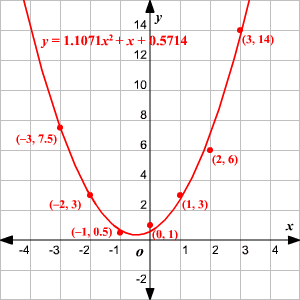
\includegraphics[width=0.42\textwidth]{images/quadratic-regression.png}
\caption{Quadratic Regression (Nguồn: Varsity Tutors).}
\label{fig:quadratic}
\end{figure}

\subsection{Hạn chế của Linear Regression}

Hạn chế đầu tiên của Linear Regression là nó rất \textbf{nhạy cảm với nhiễu}
(sensitive to noise). Trong ví dụ về mối quan hệ giữa chiều cao và cân nặng
bên trên, nếu có chỉ một cặp dữ liệu \emph{nhiễu} (150 cm, 90 kg) thì kết quả
sẽ sai khác đi rất nhiều. Xem hình dưới đây:

\begin{figure}[htbp]
\centering
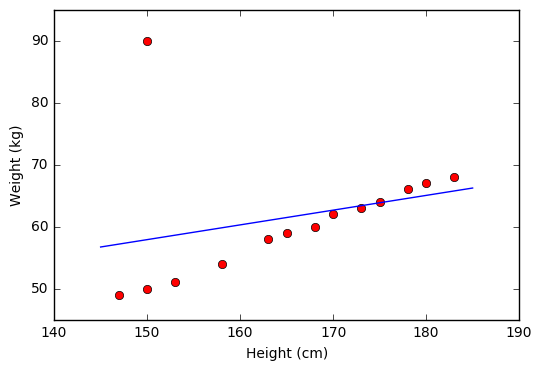
\includegraphics[width=0.72\textwidth]{images/output_13_1.png}
\caption{Ảnh hưởng của một điểm dữ liệu nhiễu tới đường hồi quy.}
\label{fig:noise}
\end{figure}

Vì vậy, trước khi thực hiện Linear Regression, các nhiễu (\emph{outlier}) cần
phải được loại bỏ. Bước này được gọi là tiền xử lý (pre-processing).

Hạn chế thứ hai của Linear Regression là nó \textbf{không biểu diễn được các
mô hình phức tạp}. Mặc dù trong phần trên, chúng ta thấy rằng phương pháp này
có thể được áp dụng nếu quan hệ giữa \emph{outcome} và \emph{input} không
nhất thiết phải là tuyến tính, nhưng mối quan hệ này vẫn đơn giản nhiều so với
các mô hình thực tế. Hơn nữa, chúng ta sẽ tự hỏi: làm thế nào để xác định được
các hàm $x_1^2, \sin(x_2), x_1x_2$ như ở trên?

\subsection{Các phương pháp tối ưu}

Linear Regression là một mô hình đơn giản, lời giải cho phương trình đạo hàm
bằng 0 cũng khá đơn giản. Trong hầu hết các trường hợp, chúng ta không thể
giải được phương trình đạo hàm bằng 0.

Nhưng có một điều chúng ta nên nhớ: \textbf{còn tính được đạo hàm là còn có
hy vọng}.

\renewcommand{\refname}{Tài liệu tham khảo}
\phantomsection
\addcontentsline{toc}{section}{Tài liệu tham khảo}
\begin{thebibliography}{3}\raggedright
\bibitem{wikipedia}
Linear Regression -- Wikipedia.
\url{https://en.wikipedia.org/wiki/Linear_regression}.

\bibitem{mastery}
Simple Linear Regression Tutorial for Machine Learning.
\url{http://machinelearningmastery.com/simple-linear-regression-tutorial-for-machine-learning/}.

\bibitem{pseudoinverse}
Least Squares, Pseudo-Inverses, PCA \& SVD.
\url{http://www.sci.utah.edu/~gerig/CS6640-F2012/Materials/pseudoinverse-cis61009sl10.pdf}.
\end{thebibliography}

\end{document}
